\section{Prinzip von Coupled-Line-Filtern}
Ein Coupled Line Filter besteht aus zwei Parallelen Übertragungsleitungen (Transmission Lines), 
diese liegen so nahe beieinander, dass ihre elektromagnetischen Felder sich gegenseitig beeinflussen.
Diese elektromagnetische Kopplung hat Induktive sowie Kapazitive Anteile.
\\
Wird ein Hochfrequenzsignal über ein Coubled line Filter übertragen, hängt es stark
von der Frequenz des Signals ab, wie viel Leistung am Ausgang ankommt.
Da je nach Frequenz der Energieaustausch zwischen den Gekoppelten Leitungen effizienter oder weniger effizient ist.
Das kann man sich jedoch zu nutze machen, um gewünsche Frequenzen duch den Filter zu lassen und ungewünschte zu dämpfen bzw. sperren.

\section{Eigenschaften von Microstrip-Leitungen}
Microstip(Streifenleitung) gehören zu einer bestimmten Klasse der Wellenleiter.
Besonders in der Hochfrequenztechnik kommen sie zum Einsatz.
Um eine Microstrip-Leitung zu bauen, wird ein dünner Leitfähiger Streifen, wie Kupfer, auf einem Dielektrikum, wie FR4, aufgebracht.
\section{Charakteristische Leitungslänge und Filterordnung}

\section{Bedeutung der S-Parameter}
S-Parameter bzw. Streuparameter werden genutzt, um die HF-Eigenschaften eines
Netzwerks darzustellen. Sie werden benötigt, um zu verstehen, welche Anteile eines Signals
reflektiert, durchgelassen oder zwischen den Ports eines Netzwerks übertragen werden.
Sie werden komplex dargestellt, also mit Betrags- und Phasenkomponente.

Die Indexnummerierung folgt dem Energiefluss:

\begin{itemize}
    \item Verläuft die Energie von Port 1 zu Port 1, heißt der S-Parameter S11.
    \item Verläuft die Energie von Port 2 zu Port 1, heißt der S-Parameter S21.
\end{itemize}
Somit können an einem Zweitor folgende S-Parameter auftreten:
\begin{itemize}
    \item S11 ist der Eingangsreflexionsfaktor. Dieser Parameter gibt an, wie viel des Eingangssignals zurückreflektiert wird.
    \item S21 ist der Vorwärtstransmissionsfaktor. Dieser Parameter gibt die Effizienz der Signalübertragung vom Eingang zum Ausgang an.
    \item S12 ist der Rückwärtstransmissionsfaktor. Dieser Parameter gibt an, wie gut Port 1 von Signalen von Port 2 isoliert ist.
    \item S22 ist der Ausgangsreflexionsfaktor. Dieser Parameter gibt an, wie viel des Ausgangssignals zurückreflektiert wird.
\end{itemize}

\subsection{Smith-Diagramm}
Das Smith-Diagramm ermöglicht die grafische Darstellung der S-Parameter.
Dafür werden der Real- und Imaginärteil des Reflexionsfaktors in Abhängigkeit von der Frequenz
aufgetragen und ermöglichen dadurch eine einfachere Impedanzanpassung.
\begin{figure}[h]
    \centering
    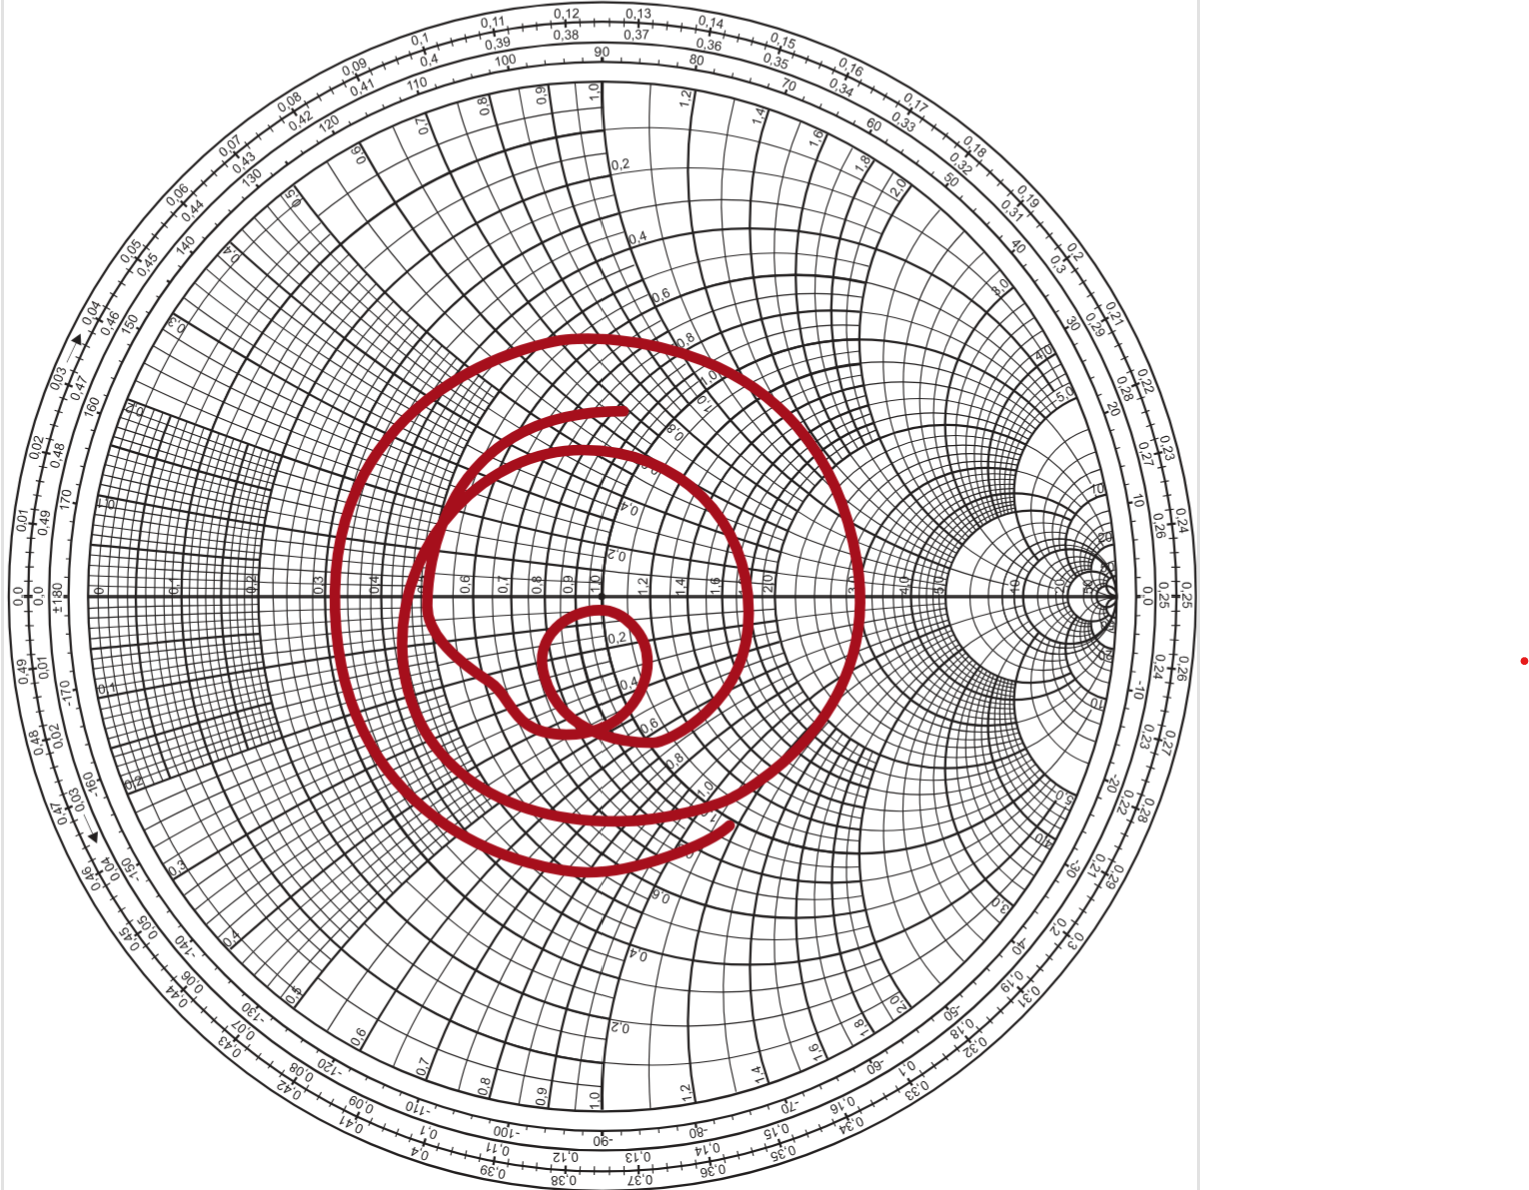
\includegraphics[width=0.4\textwidth]{Pictures/SmithDiagram.png}
    \caption{Smith-Diagramm Beispiel}
    \footnotesize{Quelle: \url{https://www.rohde-schwarz.com/de/produkte/messtechnik/essentials-test-equipment/spectrum-analyzers/s-parameter-verstehen_257831.html#gallery-13}}
\end{figure}

\clearpage